
\documentclass[12pt,hyperref={CJKbookmarks=true}]{beamer} %14pt为字体尺寸,默认值11pt.有8-12;14;17;20;bigger;smaller
%%%%%%%%%%%%%%%%%%%%%%%%%%%%%%%%%%%%%%%%%
% 模板資訊:
% 模板名稱:Beamer
% 版本:1.0 (2023.07.09)
% 修改者:Ernie
% 編譯器:XeLaTeX
%
% 原始模板的資訊:
% 模板名稱:Beamer Presentation
% 作者:Vel (vel@latextemplates.com)
% 編譯器:XeLaTeX
% 授權:CC BY-NC-SA 4.0 (https://creativecommons.org/licenses/by-nc-sa/4.0/)
% 下載連結:https://www.LaTeXTemplates.com
%
% 製作本模板之目的:
% 為了讓 LaTeX 初學者能夠輕鬆地完成專業的學術簡報,因此我針對 Vel 製作的模板做了大幅度的修改及附上清楚明瞭的註解。
%
% 如果您有任何問題,可以透過 Email 聯繫我們:stateconlab@gmail.com
% 
% p.s. 也別忘了關注我們的 YouTube、IG 和 Medium 喔!
% 1. YouTube:https://www.youtube.com/@StatEconLab
% 2. IG:https://www.instagram.com/stateconlab
% 3. Mediun:https://medium.com/@stateconlab
%%%%%%%%%%%%%%%%%%%%%%%%%%%%%%%%%%%%%%%%%

%----------------------------------------------------------------------------------------
%	封包與文檔配置
%----------------------------------------------------------------------------------------

\usepackage[space,noindent]{ctex}

% 自訂字體顏色的封包
\usepackage{xcolor} 

%% 自訂顏色

\definecolor{pbblue}{HTML}{0A75A8}% color for the progress bar and the circle
% 數學工具及符號
%\usepackage{mathtools, amsmath, amsfonts, amsthm, latexsym} 

% 分別將數學符號間的間隔加大及加粗
%\usepackage{newtxtext,newtxmath}

% 圖表自動編號的封包
%\usepackage{caption} 

%% 設定自動編號
%\setbeamertemplate{caption}[numbered]

%% 設定圖表編號及標籤的字體大小及字形
%\captionsetup[figure]{font=small, labelfont=md}
%\captionsetup[table]{font=small, labelfont=md}

% 導入圖形與表格的封包
%\usepackage{graphicx}  % \scalebox{} 可用於將過大的表格縮小
%\usepackage{booktabs}

% 排列多個子圖形的封包
%\usepackage{subfigure} 

% 允許表格的一格能多列呈現的封包
%\usepackage{multirow} 

% 可指定表格排版的封包
%\usepackage{array}

% 翻轉表格的封包
%\usepackage{lscape} 

% 序列標號
%\usepackage{enumerate} 

% 繪圖封包 (用於添加浮水印)
\usepackage{tikz}

% 引注參考資料
%\usepackage{natbib}

% 註釋掉大部分的封包
%\usepackage{comment}

\usetikzlibrary{shapes,fit,calc,positioning}

% 設定中文的標籤
%\renewcommand{\figurename}{圖} 
\renewcommand{\tablename}{表} 

%----------------------------------------------------------------------------------------
%	排版形式 (擇一,不選等同選擇默認的排版形式)
%----------------------------------------------------------------------------------------

%\mode<presentation>{
%\usetheme{default}
%\usetheme{AnnArbor}
%\usetheme{Antibes}
%\usetheme{Bergen}
%\usetheme{Berkeley}%演示主题为侧边导航条
%\usetheme{Berlin}
\usetheme{Boadilla}%蓝色主题
%\usetheme{CambridgeUS}
%\usetheme{Copenhagen}
%\usetheme{Darmstadt}
%\usetheme{Dresden}
%\usetheme{Frankfurt}
%\usetheme{Goettingen}
%\usetheme{Hannover}
%\usetheme{Ilmenau}
%\usetheme{JuanLesPins}
%\usetheme{Luebeck}
%\usetheme{Madrid}
%\usetheme{Malmoe}
%\usetheme{Marburg}
%\usetheme{Montpellier}
%\usetheme{PaloAlto}
%\usetheme{Pittsburgh}
%\usetheme{Rochester}
%\usetheme{Singapore}
%\usetheme{Szeged}
%\usetheme{Warsaw}

%----------------------------------------------------------------------------------------
%	外框形式 (擇一,不選等同選擇默認的外框形式)
%----------------------------------------------------------------------------------------

%\useoutertheme{default}
%\useoutertheme{infolines}
%\useoutertheme{miniframes}
%\useoutertheme{smoothbars}
%\useoutertheme{sidebar}
%\useoutertheme{split}
%\useoutertheme{shadow}
%\useoutertheme{tree}
%\useoutertheme{smoothtree}

%----------------------------------------------------------------------------------------
%	外框的自訂義調整 
%----------------------------------------------------------------------------------------

% 外框上緣的字 (fg) 為黑色,背景 (bg) 為白色。
%\setbeamercolor{section in head/foot}{fg=white, bg=black} 

% 外框上緣顯示的章節(section)頁數標籤是否關閉
%\setbeamertemplate{mini frames}{}   

% 調整外框形式的字體大小
%\setbeamerfont{headline}{size=\scriptsize}
%\setbeamerfont{footline}{size=\scriptsize}

% 取消右下方的跳轉工具列
\setbeamertemplate{navigation symbols}{} 

%% 自定義1:外框下緣僅出現名字及頁碼
%\setbeamertemplate{footline}
%{\leavevmode%
%\hbox{%
%\begin{beamercolorbox}[wd=0.5\paperwidth,ht=3ex,dp=1ex,leftskip=2ex]%
%{author in head/foot}%
%{\footnotesize\textbf{\insertshortauthor}}%
%\end{beamercolorbox}%
%\begin{beamercolorbox}[wd=0.5\paperwidth,ht=3ex,dp=1ex,right]%
%{author in head/foot}%
%\footnotesize \textbf{{\insertframenumber{} / \inserttotalframenumber\hspace*{2ex}}} %頁碼控制選項
%\end{beamercolorbox}%
%}}

%% 自定義2:清除外框下緣但僅出頁碼
%\setbeamertemplate{footline}[page number] 

%% 自定義3:清除外框下緣
%\setbeamertemplate{footline}[] 

%----------------------------------------------------------------------------------------
%	顏色主題 (擇一,不選等同選擇默認的顏色主題)
%----------------------------------------------------------------------------------------

%\usecolortheme{default}
%\usecolortheme{albatross}
%\usecolortheme{beaver}
%\usecolortheme{beetle}
%\usecolortheme{crane}
%\usecolortheme{dolphin}
%\usecolortheme{dove}
%\usecolortheme{fly}
%\usecolortheme{lily}
%\usecolortheme{orchid}
%\usecolortheme{rose}
%\usecolortheme{seagull}
%\usecolortheme{seahorse}
\usecolortheme{whale}%颜色主题为
%\usecolortheme{wolverine}

%----------------------------------------------------------------------------------------
%	顏色主題的自訂義調整 
%----------------------------------------------------------------------------------------

% 全文的主題色 (可以特別針對報告對象或機構的代表色調整!)
%\setbeamercolor{structure}{fg=Myblue} 

% 封面頁中標題區塊的底色及字體顏色
%\setbeamercolor{title}{bg=green, fg=black} 

% 各頁標題區塊的底色及字體顏色
%\setbeamercolor{frametitle}{bg=white,fg=black} 

% 全文的內文顏色
%\setbeamercolor{normal text}{fg=orange}

% 數學區塊的標題顏色 
%\setbeamercolor{block title}{bg=blue,fg=yellow} 

% 數學區塊的內文顏色 
%\setbeamercolor{block body}{bg=green,fg=red} 

% 警示文字的顏色
%\setbeamercolor{alerted text}{fg=red} 

%----------------------------------------------------------------------------------------
%	enumerate 及 item 的形狀
%----------------------------------------------------------------------------------------

%\useinnertheme{rounded} % 圓球 (3D)
%\useinnertheme{circles} % 圓形 (2D)
%\useinnertheme{rectangles} % 方形
%\useinnertheme{triangle} % 三角形
%\useinnertheme{inmargin} % 插入邊沿
%\setbeamertemplate{itemize items}[triangle]

%----------------------------------------------------------------------------------------
%	自訂 item 的顏色
%----------------------------------------------------------------------------------------

%\setbeamercolor{item projected}{bg=red}

%----------------------------------------------------------------------------------------
%	個人化的設置及細節調整
%----------------------------------------------------------------------------------------

% 設定頁面邊界
%\setbeamersize{text margin left=0.6cm, text margin right=0.6cm}
%\special{papersize=\the\paperwidth,\the\paperheight}
%\providecommand{\tabularnewline}{\\}
%}

%----------------------------------------------------------------------------------------
%	個人化的背景調控
%----------------------------------------------------------------------------------------

% 背景照片設置
%\setbeamertemplate{background}{\includegraphics[height=\paperheight]{Fig/Background.png}}

% 浮水印設定
%\usebackgroundtemplate{%
%	\tikz[overlay, remember picture] % 讓 logo 能每頁都顯示
%	\node[opacity=0.3, below=-1.25cm, at=(current page.center)] % 調整透明度 (opacity) 及浮水印的位置
%	{\includegraphics[scale = 0.14]{Fig/nthulogo.png}}; % 載入 logo 及調整大小
%	}
 % 載入封包與文檔配置
\usepackage{verbatim}
%\usepackage{multicol}分栏
\usepackage{tikz}
\usetikzlibrary{backgrounds,circuits.ee.IEC.relay}
%\usepackage[autoplay,loop]{animate}
\usepackage{animate}
\tikzset{
dpu/.style={rectangle,rounded corners=2pt,
minimum width=35pt,minimum height=40pt,inner sep=5pt,
draw=black,fill=black!20,scale=0.8},
switch/.style={rectangle,rounded corners=5pt,
minimum width=15pt,minimum height=50pt,inner sep=5pt,
draw=black,fill=black!20}
}




\makeatletter
\def\progressbar@progressbar{} % the progress bar
\newcount\progressbar@tmpcounta% auxiliary counter
\newcount\progressbar@tmpcountb% auxiliary counter
\newdimen\progressbar@pbht %progressbar height
\newdimen\progressbar@pbwd %progressbar width
\newdimen\progressbar@rcircle % radius for the circle
\newdimen\progressbar@tmpdim % auxiliary dimension

\progressbar@pbwd=\linewidth
\progressbar@pbht=1pt
\progressbar@rcircle=2.5pt

% the progress bar
\def\progressbar@progressbar{%

    \progressbar@tmpcounta=\insertframenumber
    \progressbar@tmpcountb=\inserttotalframenumber
    \progressbar@tmpdim=\progressbar@pbwd
    \multiply\progressbar@tmpdim by \progressbar@tmpcounta
    \divide\progressbar@tmpdim by \progressbar@tmpcountb

  \begin{tikzpicture}
    \draw[pbblue!30,line width=\progressbar@pbht]
      (0pt, 0pt) -- ++ (\progressbar@pbwd,0pt);

    \filldraw[pbblue!30] %
      (\the\dimexpr\progressbar@tmpdim-\progressbar@rcircle\relax, .5\progressbar@pbht) circle (\progressbar@rcircle);

    \node[draw=pbblue!30,text width=4em,align=center,inner sep=1pt,
      text=pbblue!70,anchor=east] at (0,0) {\textnormal{%
             \pgfmathparse{\insertframenumber*100/\inserttotalframenumber}%
             \pgfmathprintnumber[fixed,precision=2]{\pgfmathresult}\,\%%
        }%
};
  \end{tikzpicture}%
}

\addtobeamertemplate{headline}{}
{%
  \begin{beamercolorbox}[wd=\paperwidth,ht=4ex,center,dp=1ex]{white}%
    \progressbar@progressbar%
  \end{beamercolorbox}%
}
\makeatother








\begin{document}
	
	\kaishu
	
	\title{吹灰器控制原理培训}
\subtitle{本体吹灰}
	\author{热控专业}
	\institute[检修部热控班组]{热控班组}
	\date{\today}
	\begin{frame}
		\titlepage
	\end{frame}
\begin{frame}{\textbf{目录}}
\tableofcontents
\end{frame}
	\section{吹灰器简介}
	\subsection{吹灰器作用及工作原理}
\begin{frame}{吹灰器作用及工作原理}{吹灰器作用}
\begin{block}{吹灰系统设置背景}
			 锅炉受热面上积灰是常见的现象。由于灰的导热系数小,因此积灰使热阻增加,热交换恶化,以至排烟温度升高,锅炉效率降低。积灰严重而形成堵灰时,会增加烟道阻力,使锅炉出力降低,甚至被迫停炉清理。
		\end{block}
\begin{exampleblock}{吹灰器作用}
主要用于锅炉水冷壁的吹扫,避免向火面积灰和结渣,提高热效率,为锅炉满负荷、长周期的正常运行提供必要的保证。
		\end{exampleblock}
		
	\end{frame}
\begin{frame}{吹灰器作用及工作原理}{吹灰器工作原理}
\begin{block}{吹灰器工作原理}
			从伸缩旋转的吹灰抢管端部的两个或几个喷嘴中,喷出蒸汽或压缩空气持续冲击、清洗受热面
		\end{block}
\begin{exampleblock}{吹灰器工作过程}
吹灰周期从吹灰枪处在起始位置时开始。吹灰器启动后,电动机驱动跑车沿着梁两侧的导轨前移,将吹灰枪匀速旋入锅炉内。喷嘴进入炉内一定距离后,跑车开启阀门,吹灰开始。跑车继续前进,吹灰枪不断旋转、前进吹灰;直至到达前端极限后,电动机反转,跑车退回,吹灰枪管以与前进时不同轨迹后退吹灰。当喷嘴接近炉墙时,阀门关闭,吹灰停止。跑车继续后退回到起始位置。
		\end{exampleblock}
	\end{frame}
\subsection{我厂吹灰器介绍}
\begin{frame}{我厂吹灰器简介}{吹灰器分类}
\begin{block}{吹灰器分类-工作方式}
				\begin{enumerate}
				\item  伸缩式吹灰器:跑车采用双齿条传动,直线进退到位。
				
				\item  炉膛吹灰器:伸缩旋转进到位后再反向旋转退到位。
				
				\item   固定式吹灰器:单向固定旋转,一个限位开关。
				
			\end{enumerate}
		\end{block}
\begin{exampleblock}{吹灰器分类-工艺系统}
\begin{enumerate}
				\item  本体吹灰器:炉膛吹灰配置总计65台。
				
				\item  空预器吹灰器:单独配置上下两层共4台伸缩式吹灰器。
				
				\item   脱硝吹灰器:单独配置9台伸缩式吹灰器。
				
			\end{enumerate}
		\end{exampleblock}
		
	\end{frame}
\begin{frame}{我厂吹灰器简介}{本体吹灰器布置}
\begin{block}{吹灰器布置:炉膛吹灰配置总计65台}
				\begin{enumerate}
				\item  空预器烟道(21m层)12台,四周布置,每侧3台,短吹
				
				\item  省煤器(25m层)12台,四周布置,每侧3台,短吹
				
				\item   省煤器(28m层)12台,四周布置,每侧3台,短吹
\item   省煤器(31m层)6台,两侧布置,每侧3台,中长吹
\item   省煤器(33m层)6台,两侧布置,每侧3台,长吹
\item   过热器(40m层)8台,两侧布置,每侧4台,长吹
				
			\end{enumerate}

		\end{block}

	\end{frame}
\section{锅炉本体吹灰器电气原理}
	\subsection{锅炉本体吹灰器动力回路}
	\begin{frame}{锅炉本体吹灰器动力回路}{锅炉本体吹灰器动力回路}
		\begin{columns}
			\column{.5\textwidth}
		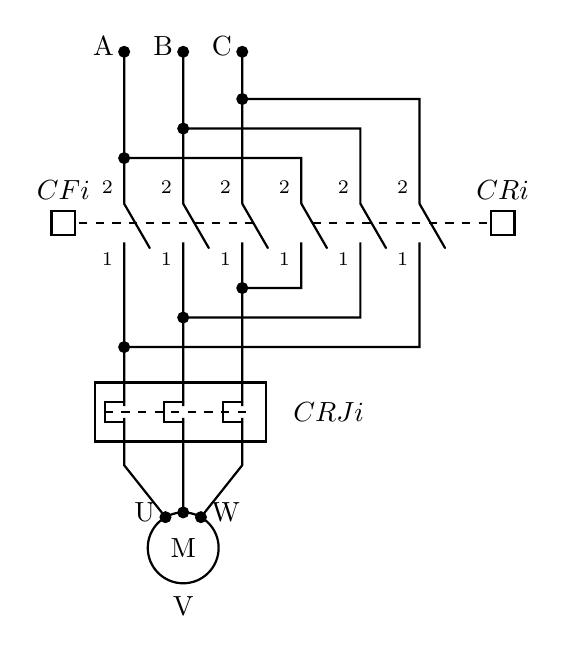
\begin{tikzpicture}[circuit ee IEC relay,thick,scale=1.5]
\draw (0.5,-0.7) ++(120:0.3)
node [contact,name=U,info={[left]:U}]{};
\draw (0.5,-0.7) ++(90:0.3)
node [contact,name=V,info={[below=1]:V}]{};
\draw (0.5,-0.7) ++(60:0.3)
node [contact,name=W,,info={[right]:W}]{};
\draw (0.5,-0.7) circle (0.3);
\node at(0.5,-0.7) {M};

\draw (0,3.5) node [contact,name=A,info={[left]:A}]{} -- ++(0,-0.9)
node [contact,name=A1]{} -- ++(0,-0.3)
to [make contact={term=1,term'=2}] ++(0,-0.5) -- ++(0,-0.8)
node [contact,name=A2]{}  -- ++(0,-0.5)
to [thermic sensor={name=FR}] ++(0,-0.1) -- ++(0,-0.4)
to (U);

\draw (0.5,3.5) node [contact,name=B,info={[left]:B}]{} -- ++ (0,-0.65)
node [contact,name=B1]{}  -- ++(0,-0.55)
to [make contact={term=1,term'=2}] ++(0,-0.5) -- ++(0,-0.55)
node [contact,name=B2]{} -- ++(0,-0.75)
to [thermic sensor] ++(0,-0.1) -- ++(0,-0.4)
to (V);

\draw (1,3.5) node [contact,name=C,info={[left]:C}]{} -- ++ (0,-0.4)
node [contact,name=C1]{}  -- ++(0,-0.8)
to [make contact={name=KM1,term=1,term'=2}] ++(0,-0.5) -- ++(0,-0.3)
node [contact,name=C2]{} -- ++(0,-1)
to [thermic sensor={info={[right=0.5cm]:$CRJi$}}] ++(0,-0.1) -- ++(0,-0.4)
to (W);
\draw (-0.25,0.2) rectangle (1.2,0.7);

\draw (A1) -- ++(1.5,0) -- ++(0,-0.3)
to [make contact={name=KM2,term=1,term'=2}] ++(0,-0.5) -- ++(0,-0.3) -- (C2);

\draw (B1) -- ++(1.5,0) -- ++(0,-0.55)
to [make contact={term=1,term'=2}] ++(0,-0.5) -- ++(0,-0.55) -- (B2);

\draw (C1) -- ++(1.5,0) -- ++(0,-0.8)
to [make contact={term=1,term'=2}] ++(0,-0.5) -- ++(0,-0.8) -- (A2);

\draw[dashed](KM1.mid) -- ++(-1.5,0)
node[left,draw,solid,minimum size=3mm,label={[above]:$CFi$}]{};

\draw[dashed](KM2.mid) -- ++(1.5,0)
node[right,draw,solid,minimum size=3mm,label={[above]:$CRi$}]{};

\draw[dashed](FR.mid) -- ++(1.2,0);




	\end{tikzpicture}
			\column{.4\textwidth}
\begin{block}{动力回路设备}
				\begin{enumerate}
				\item  交流接触器(CFi)
\begin{enumerate}
				\item  辅助触点为NC
				\item  线圈A1、A2接线
				\end{enumerate}
				\item  热继电器(CRJi)
\begin{enumerate}
				\item  动作电流定值
				\item  复位方式(H/A)
				\end{enumerate}
				\item  电机(M)
\begin{enumerate}
				\item  额定电流
				\item  接线方式(Y/)
				\end{enumerate}
\item  相序-正反转
				\end{enumerate}
\end{block}
		\end{columns}
	\end{frame}
\subsection{锅炉本体吹灰器控制回路}
	\begin{frame}{锅炉本体吹灰器电气原理}{锅炉本体吹灰器控制回路}
		\begin{columns}
			\column{.7\textwidth}
		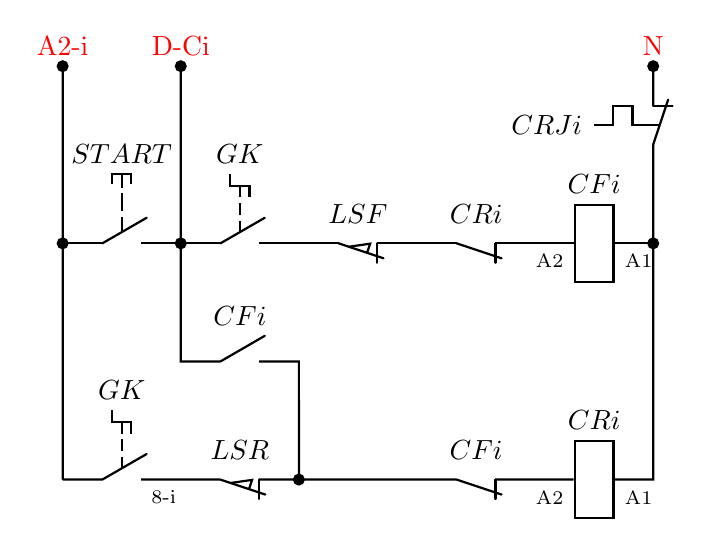
\begin{tikzpicture}[circuit ee IEC relay,thick,scale=1.5]
		
		

		\draw (0,0)
		to [make contact={turn switch={info=$GK$},term=8-i}] ++(1,0)
		to [break contact={position switch={info=$LSR$}}] ++(1,0)
		node [contact,name=A1]{} -- ++(1,0)
		to [break contact={info=$CFi$}] ++(1,0)
		to [relay coil={info=$CRi$,term=A1,term'=A2}] ++(1,0) -- ++(0,2.5)
		to [break contact={thermal switch={info=$CRJi$}}] ++(0,1)node [contact,name=N]{}
		++(-4,0)node [contact,name=Di]{}
++(-1,0)node [contact,name=L]{} to (0,0);

		\draw (0,2) node[contact]{}
		to [make contact={push button={info=$START$}}] ++(1,0)
		node [contact,name=B1]{}
		to [make contact={turn switch={info=$GK$}}] ++(1,0)
		to [break contact={position switch={info=$LSF$}}] ++(1,0)
		to [break contact={info=$CRi$}] ++(1,0)
		to [relay coil={info=$CFi$,term=A1,term'=A2}] ++(1,0)
		node [contact,name=B2]{};
		
		\draw (Di) -- (B1) -- ++(0,-1) to [make contact={info=$CFi$}] ++(1,0) -- (A1);
		
\node[above,red] at(N) {N};
\node[above,red] at(L) {A2-i};
\node[above,red] at(Di) {D-Ci};





	\end{tikzpicture}
			\column{.3\textwidth}
\begin{block}{控制回路设备}
				\begin{enumerate}
				\item  启动按钮START
\item  DCS启动脉冲
				\item  钮子开关GK
				\item  前进限位LSF
\item  后退限位LSR
\item  进接触器CFi
\item  退接触器CRi
\item  热继电器CRJi
				\end{enumerate}
\end{block}
		\end{columns}
	\end{frame}
\begin{frame}{锅炉本体吹灰器控制原理演示}{锅炉本体吹灰器控制原理演示}
  		\begin{center}
 			\begin{animateinline}[loop, poster = first, controls, palindrome,
    				begin={\begin{tikzpicture}[circuit ee IEC relay,thick,x=8\tikzcircuitssizeunit,y=3.5\tikzcircuitssizeunit]},
    				end={\end{tikzpicture}}
			]{2}
				\node at (2.5,6) {吹灰器各元器件原始状态};
				%第一帧:吹灰器各元器件原始状态
				\draw (0,0)
				to [make contact={turn switch={info=$GK$},term=8-i}] ++(1,0)
				to [break contact={position switch={info=$LSR$}}] ++(1,0) node [contact,name=A1]{}
				to [break contact={info=$CFi$}] ++(2,0)
				to [relay coil={info=$CRi$,term=A1,term'=A2}] ++(1,0) -- ++(0,4)
				to [break contact={thermal switch={info=$CRJi$}}]++(0,1) node [contact,name=N]{}
				++(-4,0)node [contact,name=Di]{}
				++(-1,0)node [contact,name=L]{} to (0,0);

				\draw (0,3) node[contact]{}
				to [make contact={push button={info=$START$}}] ++(1,0) node [contact,name=B1]{}
				to [make contact={turn switch={info=$GK$}}] ++(1,0)
				to [break contact={position switch={info=$LSF$}}] ++(1,0)
				to [break contact={info=$CRi$}] ++(1,0)
				to [relay coil={info=$CFi$,term=A1,term'=A2}] ++(1,0) node [contact,name=B2]{};
		
				\draw (Di) -- (B1) -- ++(0,-1.5) to [make contact={info=$CFi$}] ++(1,0) -- (A1);
		
				\node[above,red] at(N) {N};
				\node[left,red] at(L) {A2-i};
				\node[left,red] at(Di) {D-Li};
				\newframe
				\node at (2.5,6) {吹灰器退到位,急停旋钮旋至复位位};
				%第二帧:吹灰器退到位,急停旋钮旋至复位位
				\draw (0,0)
				to [make contact={turn switch={info=$GK$},activated,term=8-i}] ++(1,0)
				to [break contact={position switch={info=$LSR$},activated}] ++(1,0) node [contact,name=A1]{}
				to [break contact={info=$CFi$}] ++(2,0)
				to [relay coil={info=$CRi$,term=A1,term'=A2}] ++(1,0) -- ++(0,4)
				to [break contact={thermal switch={info=$CRJi$}}]++(0,1) node [contact,name=N]{}
				++(-4,0)node [contact,name=Di]{}
				++(-1,0)node [contact,name=L]{} to (0,0);

				\draw (0,3) node[contact]{}
				to [make contact={push button={info=$START$}}] ++(1,0) node [contact,name=B1]{}
				to [make contact={turn switch={info=$GK$},activated}] ++(1,0)
				to [break contact={position switch={info=$LSF$}}] ++(1,0)
				to [break contact={info=$CRi$}] ++(1,0)
				to [relay coil={info=$CFi$,term=A1,term'=A2}] ++(1,0) node [contact,name=B2]{};
		
				\draw (Di) -- (B1) -- ++(0,-1.5) to [make contact={info=$CFi$}] ++(1,0) -- (A1);
		
				\node[above,red] at(N) {N};
				\node[left,red] at(L) {A2-i};
				\node[left,red] at(Di) {D-Li};
				\newframe
				\node at (2.5,6) {按下启动按钮后,吹灰器开始前进,退到位限位开关未脱开前};
				%第三帧:按下启动按钮后,吹灰器开始前进,退到位限位开关未脱开前
				\draw (0,0)
				to [make contact={turn switch={info=$GK$},activated,term=8-i}] ++(1,0)
				to [break contact={position switch={info=$LSR$},activated}] ++(1,0) node [contact,name=A1]{}
				to [break contact={info=$CFi$},activated] ++(2,0)
				to [relay coil={info=$CRi$,term=A1,term'=A2}] ++(1,0) -- ++(0,4)
				to [break contact={thermal switch={info=$CRJi$}}]++(0,1) node [contact,name=N]{}
				++(-4,0)node [contact,name=Di]{}
				++(-1,0)node [contact,name=L]{} to (0,0);

				\draw[red] (0,3) node[contact]{}
				to [make contact={push button={info=$START$},activated}] ++(1,0) node [contact,name=B1]{}
				to [make contact={turn switch={info=$GK$},activated}] ++(1,0)
				to [break contact={position switch={info=$LSF$}}] ++(1,0)
				to [break contact={info=$CRi$}] ++(1,0)
				to [relay coil={info=$CFi$,{fill=red},term=A1,term'=A2}] ++(1,0) node [contact,name=B2]{};
		
				\draw (Di) -- (B1) -- ++(0,-1.5) to [make contact={info=$CFi$},activated] ++(1,0) -- (A1);
		
				\node[above,red] at(N) {N};
				\node[left,red] at(L) {A2-i};
				\node[left,red] at(Di) {D-Li};
				\newframe
				\node at (2.5,6) {吹灰器前进,退到位限位开关脱开,开始按钮未放开};
				%第四帧:吹灰器开始前进,退到位限位开关脱开,开始按钮未放开
				\draw[red] (0,0)
				to [make contact={turn switch={info=$GK$},activated,term=8-i}] ++(1,0)
				to [break contact={position switch={info=$LSR$}}] ++(1,0) node [contact,name=A1]{};
				\draw (A1) to [break contact={info=$CFi$},activated] ++(2,0)
				to [relay coil={info=$CRi$,term=A1,term'=A2}] ++(1,0) -- ++(0,4)
				to [break contact={thermal switch={info=$CRJi$}}]++(0,1) node [contact,name=N]{}
				++(-4,0)node [contact,name=Di]{}
				++(-1,0)node [contact,name=L]{} to (0,0);

				\draw[red] (0,3) node[contact]{}
				to [make contact={push button={info=$START$},activated}] ++(1,0) node [contact,name=B1]{}
				to [make contact={turn switch={info=$GK$},activated}] ++(1,0)
				to [break contact={position switch={info=$LSF$}}] ++(1,0)
				to [break contact={info=$CRi$}] ++(1,0)
				to [relay coil={info=$CFi$,{fill=red},term=A1,term'=A2}] ++(1,0) node [contact,name=B2]{};
		
				\draw (Di) -- (B1);
				\draw[red] (B1) -- ++(0,-1.5) to [make contact={info=$CFi$},activated] ++(1,0) -- (A1);
				\node[above,red] at(N) {N};
				\node[left,red] at(L) {A2-i};
				\node[left,red] at(Di) {D-Li};
				\newframe
				\node at (2.5,6) {吹灰器前进,退到位限位开关脱开,开始按钮放开};
				%第五帧:吹灰器开始前进,退到位限位开关脱开,开始按钮放开
				\draw (0,0)
				to [make contact={turn switch={info=$GK$},activated,term=8-i}] ++(1,0)
				to [break contact={position switch={info=$LSR$}}] ++(1,0) node [contact,name=A1]{}
				to [break contact={info=$CFi$},activated] ++(2,0)
				to [relay coil={info=$CRi$,term=A1,term'=A2}] ++(1,0) -- ++(0,4)
				to [break contact={thermal switch={info=$CRJi$}}]++(0,1) node [contact,name=N]{}
				++(-4,0)node [contact,name=Di]{}
				++(-1,0)node [contact,name=L]{} to (0,0);

				\draw (0,3) node[contact]{}
				to [make contact={push button={info=$START$}}] ++(1,0) node [contact,name=B1]{}
				to [make contact={turn switch={info=$GK$},activated}] ++(1,0)
				to [break contact={position switch={info=$LSF$}}] ++(1,0)
				to [break contact={info=$CRi$}] ++(1,0)
				to [relay coil={info=$CFi$,{fill=red},term=A1,term'=A2}] ++(1,0) node [contact,name=B2]{};
		
				\draw (Di) -- (B1) -- ++(0,-1.5) to [make contact={info=$CFi$},activated] ++(1,0) -- (A1);
		
				\node[above,red] at(N) {N};
				\node[left,red] at(L) {A2-i};
				\node[left,red] at(Di) {D-Li};
				\newframe
				\node at (2.5,6) {吹灰器前进到位后开始后退};
				%第六帧:吹灰器前进到位后开始后退
				\draw (0,0)
				to [make contact={turn switch={info=$GK$},activated,term=8-i}] ++(1,0)
				to [break contact={position switch={info=$LSR$}}] ++(1,0) node [contact,name=A1]{}
				to [break contact={info=$CFi$}] ++(2,0)
				to [relay coil={info=$CRi$,{fill=red},term=A1,term'=A2}] ++(1,0) -- ++(0,4)
				to [break contact={thermal switch={info=$CRJi$}}]++(0,1) node [contact,name=N]{}
				++(-4,0)node [contact,name=Di]{}
				++(-1,0)node [contact,name=L]{} to (0,0);

				\draw (0,3) node[contact]{}
				to [make contact={push button={info=$START$}}] ++(1,0) node [contact,name=B1]{}
				to [make contact={turn switch={info=$GK$},activated}] ++(1,0)
				to [break contact={position switch={info=$LSF$},activated}] ++(1,0)
				to [break contact={info=$CRi$}] ++(1,0)
				to [relay coil={info=$CFi$,term=A1,term'=A2}] ++(1,0) node [contact,name=B2]{};
		
				\draw (Di) -- (B1) -- ++(0,-1.5) to [make contact={info=$CFi$}] ++(1,0) -- (A1);
		
				\node[above,red] at(N) {N};
				\node[left,red] at(L) {A2-i};
				\node[left,red] at(Di) {D-Li};
				\newframe
				\node at (2.5,6) {吹灰器后退过程中进到位限位开关复位};
				%第七帧:吹灰器后退过程中进到位限位开关复位
				\draw (0,0)
				to [make contact={turn switch={info=$GK$},activated,term=8-i}] ++(1,0)
				to [break contact={position switch={info=$LSR$}}] ++(1,0) node [contact,name=A1]{}
				to [break contact={info=$CFi$}] ++(2,0)
				to [relay coil={info=$CRi$,{fill=red},term=A1,term'=A2}] ++(1,0) -- ++(0,4)
				to [break contact={thermal switch={info=$CRJi$}}]++(0,1) node [contact,name=N]{}
				++(-4,0)node [contact,name=Di]{}
				++(-1,0)node [contact,name=L]{} to (0,0);

				\draw (0,3) node[contact]{}
				to [make contact={push button={info=$START$}}] ++(1,0) node [contact,name=B1]{}
				to [make contact={turn switch={info=$GK$},activated}] ++(1,0)
				to [break contact={position switch={info=$LSF$}}] ++(1,0)
				to [break contact={info=$CRi$}] ++(1,0)
				to [relay coil={info=$CFi$,term=A1,term'=A2}] ++(1,0) node [contact,name=B2]{};
		
				\draw (Di) -- (B1) -- ++(0,-1.5) to [make contact={info=$CFi$}] ++(1,0) -- (A1);
		
				\node[above,red] at(N) {N};
				\node[left,red] at(L) {A2-i};
				\node[left,red] at(Di) {D-Li};
				\newframe
				\node at (2.5,5) {吹灰器后退到位};
				%第八帧:吹灰器后退到位
				\draw (0,0)
				to [make contact={turn switch={info=$GK$},activated,term=8-i}] ++(1,0)
				to [break contact={position switch={info=$LSR$},activated}] ++(1,0) node [contact,name=A1]{}
				to [break contact={info=$CFi$}] ++(2,0)
				to [relay coil={info=$CRi$,term=A1,term'=A2}] ++(1,0) -- ++(0,4)
				to [break contact={thermal switch={info=$CRJi$}}]++(0,1) node [contact,name=N]{}
				++(-4,0)node [contact,name=Di]{}
				++(-1,0)node [contact,name=L]{} to (0,0);

				\draw (0,3) node[contact]{}
				to [make contact={push button={info=$START$}}] ++(1,0) node [contact,name=B1]{}
				to [make contact={turn switch={info=$GK$},activated}] ++(1,0)
				to [break contact={position switch={info=$LSF$}}] ++(1,0)
				to [break contact={info=$CRi$}] ++(1,0)
				to [relay coil={info=$CFi$,term=A1,term'=A2}] ++(1,0) node [contact,name=B2]{};
		
				\draw (Di) -- (B1) -- ++(0,-1.5) to [make contact={info=$CFi$}] ++(1,0) -- (A1);
		
				\node[above,red] at(N) {N};
				\node[left,red] at(L) {A2-i};
				\node[left,red] at(Di) {D-Li};
 \end{animateinline}
 \end{center}

	\end{frame}
\subsection{锅炉本体吹灰器控制系统提供用户接口}
	\begin{frame}{锅炉本体吹灰器控制系统提供用户接口}{锅炉本体吹灰器反馈信号}
\begin{columns}
			\column{.5\textwidth}
		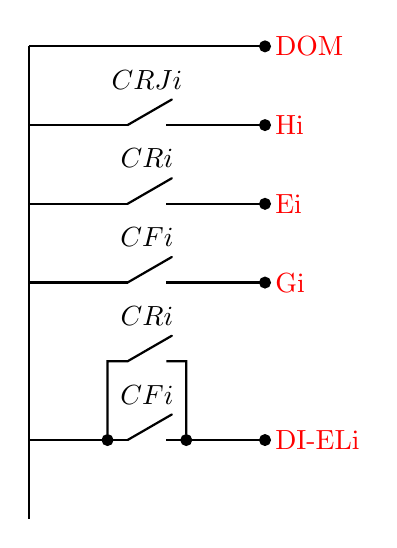
\begin{tikzpicture}[circuit ee IEC relay,thick,scale=1]
		
		
\draw (0,0) -- (0,6);
		\draw (0,1) -- ++(1,0) node [contact,name=A]{}
		to [make contact={info=$CFi$}] ++(1,0) node [contact,name=B]{} -- ++(1,0) node [contact,name=DI-ELi]{};
\draw (A) -- ++(0,1) to [make contact={info=$CRi$}] ++(1,0) -- (B);
\draw (0,3) -- ++(1,0)
		to [make contact={info=$CFi$}] ++(1,0) -- ++(1,0) node [contact,name=Gi]{};
\draw (0,4) -- ++(1,0)
		to [make contact={info=$CRi$}] ++(1,0) -- ++(1,0) node [contact,name=Ei]{};
\draw (0,5) -- ++(1,0)
		to [make contact={info=$CRJi$}] ++(1,0) -- ++(1,0) node [contact,name=Hi]{};
\draw (0,6) -- ++(3,0) node [contact,name=DOM]{};
				\node[right,red] at(DOM) {DOM};
				\node[right,red] at(Hi) {Hi};
				\node[right,red] at(Ei) {Ei};
				\node[right,red] at(Gi) {Gi};
				\node[right,red] at(DI-ELi) {DI-ELi};




	\end{tikzpicture}
			\column{.4\textwidth}
\begin{block}{反馈信号}
				\begin{enumerate}
				\item  已推进CFi
				\item  已后退CRi
				\item  已运行CFi/CRi
\item  过载CRJi
\item  电流
				\end{enumerate}
\end{block}
\begin{alertblock}{DCS/DI公共端!!!}
	DOM为DCS机柜内通道组其中一个保险端子
\end{alertblock}
		\end{columns}
	\end{frame}
\begin{frame}{锅炉本体吹灰器控制系统提供用户接口}{锅炉本体吹灰器操作指令}
\begin{columns}
			\column{.5\textwidth}
		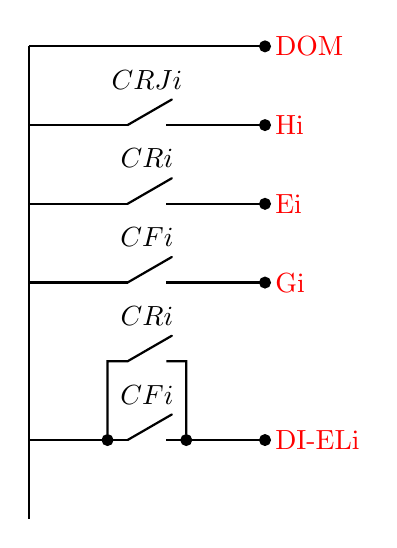
\begin{tikzpicture}[circuit ee IEC relay,thick,scale=1]
		
		
\draw (0,0) -- (0,6);
		\draw (0,1) -- ++(1,0) node [contact,name=A]{}
		to [make contact={info=$CFi$}] ++(1,0) node [contact,name=B]{} -- ++(1,0) node [contact,name=DI-ELi]{};
\draw (A) -- ++(0,1) to [make contact={info=$CRi$}] ++(1,0) -- (B);
\draw (0,3) -- ++(1,0)
		to [make contact={info=$CFi$}] ++(1,0) -- ++(1,0) node [contact,name=Gi]{};
\draw (0,4) -- ++(1,0)
		to [make contact={info=$CRi$}] ++(1,0) -- ++(1,0) node [contact,name=Ei]{};
\draw (0,5) -- ++(1,0)
		to [make contact={info=$CRJi$}] ++(1,0) -- ++(1,0) node [contact,name=Hi]{};
\draw (0,6) -- ++(3,0) node [contact,name=DOM]{};
				\node[right,red] at(DOM) {DOM};
				\node[right,red] at(Hi) {Hi};
				\node[right,red] at(Ei) {Ei};
				\node[right,red] at(Gi) {Gi};
				\node[right,red] at(DI-ELi) {DI-ELi};
		
		

	\end{tikzpicture}
			\column{.4\textwidth}
\begin{block}{DCS指令}
				\begin{enumerate}
				\item  启动D-Ci
				\item  急退HTJ
				\item  手/自动SDJ
\item  模拟MNJ
\item  控制电源ZKJ
				\end{enumerate}
\end{block}
\begin{alertblock}{启动指令脉冲时间!!!}
	启动指令脉冲时间必须满足退到位限位开关脱开
\end{alertblock}
		\end{columns}
	\end{frame}
\subsection{空预器吹灰器控制回路}
	\begin{frame}{空预器吹灰器电气原理}{空预器吹灰器控制回路}
		\begin{columns}
			\column{.7\textwidth}
		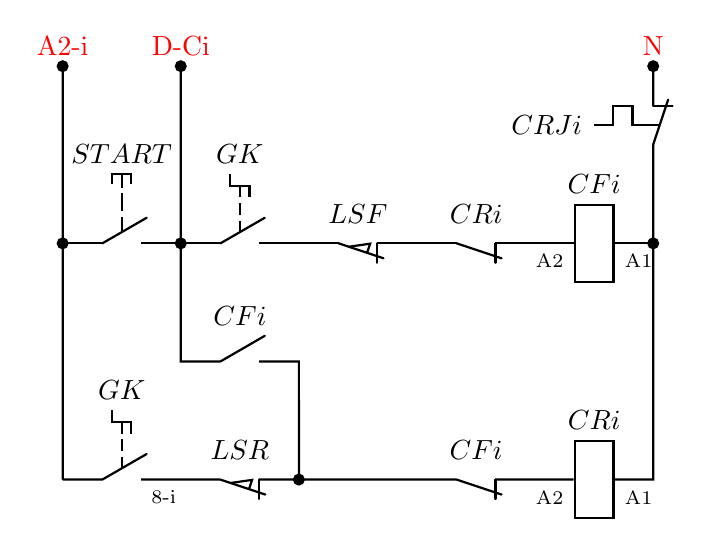
\begin{tikzpicture}[circuit ee IEC relay,thick,scale=1.5]
		
		

		\draw (0,0)
		to [make contact={turn switch={info=$GK$},term=8-i}] ++(1,0)
		to [break contact={position switch={info=$LSR$}}] ++(1,0)
		node [contact,name=A1]{} -- ++(1,0)
		to [break contact={info=$CFi$}] ++(1,0)
		to [relay coil={info=$CRi$,term=A1,term'=A2}] ++(1,0) -- ++(0,2.5)
		to [break contact={thermal switch={info=$CRJi$}}] ++(0,1)node [contact,name=N]{}
		++(-4,0)node [contact,name=Di]{}
++(-1,0)node [contact,name=L]{} to (0,0);

		\draw (0,2) node[contact]{}
		to [make contact={push button={info=$START$}}] ++(1,0)
		node [contact,name=B1]{}
		to [make contact={turn switch={info=$GK$}}] ++(1,0)
		to [break contact={position switch={info=$LSF$}}] ++(1,0)
		to [break contact={info=$CRi$}] ++(1,0)
		to [relay coil={info=$CFi$,term=A1,term'=A2}] ++(1,0)
		node [contact,name=B2]{};
		
		\draw (Di) -- (B1) -- ++(0,-1) to [make contact={info=$CFi$}] ++(1,0) -- (A1);
		
\node[above,red] at(N) {N};
\node[above,red] at(L) {A2-i};
\node[above,red] at(Di) {D-Ci};





	\end{tikzpicture}
			\column{.3\textwidth}
\begin{block}{控制回路设备}
				\begin{enumerate}
				\item  启动按钮START
\item  DCS启动脉冲
				\item  钮子开关GK
				\item  前进限位LSF
\item  后退限位LSR
\item  进接触器CFi
\item  退接触器CRi
\item  热继电器CRJi
				\end{enumerate}
\end{block}
		\end{columns}
	\end{frame}

\section{吹灰器常见故障}

\begin{frame}{吹灰器常见故障}{常见故障}
		\begin{block}{常见故障}
			\begin{enumerate}
				\item  动力回路跳闸:电缆破损接地或短路
				
				\item  电机烧损:频繁操作、接线方式错误、热继失效
				
				\item   吹灰器不动作/方向相反:动力回路缺向/相序错误
\item   接触器脱开迟缓:接触器线圈黏连
				\item  吹灰器不动作:进到为开关未复位
				\item  退到位开关未脱开就停下:脉冲指令时间过短
\item  批量吹灰器不动作:控制柜内控制回路保险烧损
.\item  批量吹灰器反馈不对:DCS侧DI通道保险烧损
			\end{enumerate}
		\end{block}

	\end{frame}



	
	

	
\begin{frame}{参考文献}
\begin{thebibliography}{10}
	
\end{thebibliography}
\end{frame}
\end{document}
